\chapter{Limits to Instruction-Level Parallelism}
\label{ch:limits_to_ilp}

The theoretical and practical bounds of Instruction-Level Parallelism (\gls{ilp}) have been the subject of extensive architectural research. Historical studies have often presented conflicting estimates regarding the maximum achievable parallelism—ranging from modest speedups of 2 to 4 in early non-speculative integer execution to theoretical gains exceeding 100 in vectorized numerical workloads. These discrepancies stem from varying assumptions regarding workload characteristics (e.g., highly parallelized FORTRAN floating-point benchmarks versus control-heavy integer C applications), compiler optimization capabilities, and available microarchitectural hardware budgets.

This chapter examines the fundamental limits of \gls{ilp}. By evaluating an idealized processor model constrained solely by true data dependencies, we establish an empirical upper bound on performance and evaluate how realistic hardware bottlenecks—such as instruction window size, finite register files, and dependency check logic—degrade throughput.

\section{The Ideal Processor Model}
\label{sec:ideal_processor_model}

To establish the absolute upper bound of \gls{ilp} inherent in application software, we define an \textbf{Ideal Processor Model}. This idealized microarchitecture eliminates all structural, control, and false data hazards, leaving true data dependencies as the sole constraint on parallel execution.

\begin{definition}{Ideal Processor Model}{ideal-processor}
An \textbf{Ideal Processor} is an unbounded theoretical execution engine characterized by the following parameters:
\begin{enumerate}
    \item \textbf{Infinite Register Renaming:} An infinite pool of physical virtual registers is available, completely eliminating Write-After-Write (\glsfmtshort{waw}) and Write-After-Read (\glsfmtshort{war}) name hazards.
    \item \textbf{Perfect Branch and Jump Prediction:} All conditional branches, indirect jumps, and procedure calls are predicted with 100\% accuracy. Branch targets are known instantaneously at Fetch, allowing instructions from arbitrary execution paths to enter the pipeline without control stalls.
    \item \textbf{Perfect Memory Alias Analysis:} The exact memory effective address of every load and store instruction is determined instantaneously. A memory load instruction can be speculatively moved ahead of preceding store instructions provided their target addresses do not conflict (no address aliasing).
    \item \textbf{Ideal Memory Hierarchy (Perfect Cache):} All memory accesses (instruction fetches and data loads/stores) hit in cache with a deterministic 1-cycle latency. Memory bandwidth and port contention are infinite.
    \item \textbf{Unbounded Execution Resources:} An infinite number of functional units and issue slots are available per cycle.
\end{enumerate}
\end{definition}

Under these idealized assumptions, all instruction execution is restricted exclusively by \glsxtrfull{raw} data dependencies. Instructions execute at the earliest possible clock cycle in which their true data operands become available.

\section{Ideal Assumptions vs. Realistic Microarchitectures}
\label{sec:ideal_vs_real}

While the ideal model provides a theoretical upper limit, physical microarchitectures operate under strict power, area, and timing constraints. Table~\ref{tab:ideal_vs_power5} contrasts the ideal model parameters against the microarchitecture of a commercial high-performance processor (IBM POWER5, 2004).

\begin{table}[htbp]
\centering
\caption{Comparison of Ideal Processor Assumptions with IBM POWER5 (2004)}
\label{tab:ideal_vs_power5}
\small
\setlength{\tabcolsep}{4pt}
\begin{tabularx}{\textwidth}{|>{\hsize=0.8\hsize}Y|>{\hsize=1.1\hsize}Y|>{\hsize=1.1\hsize}Y|}
\hline
\textbf{Architectural Feature} & \textbf{Ideal Processor Model} & \textbf{IBM POWER5 (2004)} \\ \hline
\textbf{Maximum Issue Width} & Infinite ($\infty$ inst/cycle) & 4 instructions / cycle \\ \hline
\textbf{Instruction Window} & Infinite ($\infty$ active entries) & 200 active instructions \\ \hline
\textbf{Physical Registers} & Infinite virtual register pool & 48 Integer + 40 Floating-Point \\ \hline
\textbf{Branch Prediction} & Perfect (0\% misprediction) & 2\% -- 6\% misprediction rate \\ \hline
\textbf{Cache Hierarchy Latency} & 1-cycle latency for all accesses & Multi-level (64KB L1I, 32KB L1D, 1.92MB L2, 36MB L3) \\ \hline
\textbf{Memory Alias Analysis} & Perfect dynamic disambiguation & Finite store queues with partial forwarding \\ \hline
\end{tabularx}
\end{table}

\subsection{Combinatorial Complexity of Dynamic Dependency Checking}

In a dynamic out-of-order superscalar core, evaluating data dependencies across $n$ candidate instructions within the instruction window requires pairwise comparison logic.

\begin{concept}{Combinatorial Dependency Check Complexity}{dependency-complexity}
To determine whether any pair among $n$ candidate issuing instructions exhibits a register dependency, the hardware must perform:
\begin{equation}
N_{\text{comparisons}} = n^2 - n = \mathcal{O}(n^2)
\end{equation}
parallel comparisons of destination and source register specifiers every clock cycle.
\end{concept}

This quadratic complexity creates a severe microarchitectural bottleneck:
\begin{itemize}
    \item \textbf{Small Window ($n = 50$):} Requiring $50^2 - 50 = 2{,}450$ individual comparator circuits operating within a single clock cycle.
    \item \textbf{Large Window ($n = 2{,}000$):} Requiring $2000^2 - 2000 = 3{,}998{,}000 \approx 4\text{ million}$ simultaneous comparisons per cycle.
\end{itemize}

In addition to comparison logic, physical instruction issue rates are bounded by available functional units, multi-ported register file access ports, and crossbar routing networks.

\section{Empirical Upper Limits on an Ideal Machine}
\label{sec:empirical_ideal_limits}

Figure~\ref{fig:ilp_ideal_machine} illustrates the empirical performance limits of the Ideal Processor Model across standard integer and floating-point benchmark applications.

\begin{figure}[htpb]
\centering
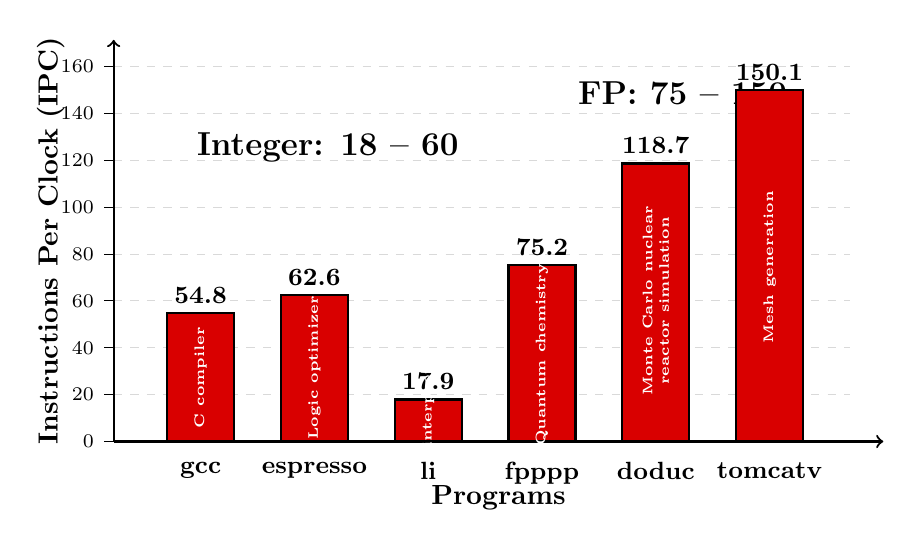
\begin{tikzpicture}[scale=0.85, font=\small]
    % Grid lines
    \draw[gray!30, dashed] (0,0) grid[ystep=0.7cm, xstep=0] (11, 5.6);
    
    % Axes
    \draw[->, thick] (0,0) -- (11.5, 0) node[below=12pt, midway, font=\bfseries] {Programs};
    \draw[->, thick] (0,0) -- (0, 6.0) node[rotate=90, above=14pt, midway, font=\bfseries] {Instructions Per Clock (IPC)};
    
    % Y-Axis Ticks & Labels (Scale: 1 unit IPC = 0.035 cm => 160 IPC = 5.6 cm)
    \foreach \y/\val in {0/0, 0.7/20, 1.4/40, 2.1/60, 2.8/80, 3.5/100, 4.2/120, 4.9/140, 5.6/160} {
        \draw (0, \y) -- (-0.15, \y) node[left, font=\scriptsize] {\val};
    }

    % Group Labels Top Text
    \node[font=\bfseries\large] at (3.2, 4.4) {Integer: 18 -- 60};
    \node[font=\bfseries\large] at (8.5, 5.2) {FP: 75 -- 150};

    % Bars (Red)
    % gcc: 54.8 IPC -> 54.8 * 0.035 = 1.918 cm
    \draw[fill=red!85!black, draw=black, thick] (0.8, 0) rectangle (1.8, 1.918);
    \node[above, font=\bfseries\small] at (1.3, 1.918) {54.8};
    \node[text=white, font=\tiny\bfseries, align=center, rotate=90] at (1.3, 0.95) {C compiler};
    \node[below=4pt, font=\bfseries\small] at (1.3, 0) {gcc};

    % espresso: 62.6 IPC -> 62.6 * 0.035 = 2.191 cm
    \draw[fill=red!85!black, draw=black, thick] (2.5, 0) rectangle (3.5, 2.191);
    \node[above, font=\bfseries\small] at (3.0, 2.191) {62.6};
    \node[text=white, font=\tiny\bfseries, align=center, rotate=90] at (3.0, 1.1) {Logic optimizer};
    \node[below=4pt, font=\bfseries\small] at (3.0, 0) {espresso};

    % li: 17.9 IPC -> 17.9 * 0.035 = 0.6265 cm
    \draw[fill=red!85!black, draw=black, thick] (4.2, 0) rectangle (5.2, 0.6265);
    \node[above, font=\bfseries\small] at (4.7, 0.6265) {17.9};
    \node[text=white, font=\tiny\bfseries, align=center, rotate=90] at (4.7, 0.31) {Lisp interpreter};
    \node[below=4pt, font=\bfseries\small] at (4.7, 0) {li};

    % fpppp: 75.2 IPC -> 75.2 * 0.035 = 2.632 cm
    \draw[fill=red!85!black, draw=black, thick] (5.9, 0) rectangle (6.9, 2.632);
    \node[above, font=\bfseries\small] at (6.4, 2.632) {75.2};
    \node[text=white, font=\tiny\bfseries, align=center, rotate=90] at (6.4, 1.3) {Quantum chemistry};
    \node[below=4pt, font=\bfseries\small] at (6.4, 0) {fpppp};

    % doduc: 118.7 IPC -> 118.7 * 0.035 = 4.1545 cm
    \draw[fill=red!85!black, draw=black, thick] (7.6, 0) rectangle (8.6, 4.1545);
    \node[above, font=\bfseries\small] at (8.1, 4.1545) {118.7};
    \node[text=white, font=\tiny\bfseries, align=center, rotate=90] at (8.1, 2.1) {Monte Carlo nuclear\\reactor simulation};
    \node[below=4pt, font=\bfseries\small] at (8.1, 0) {doduc};

    % tomcatv: 150.1 IPC -> 150.1 * 0.035 = 5.2535 cm
    \draw[fill=red!85!black, draw=black, thick] (9.3, 0) rectangle (10.3, 5.2535);
    \node[above, font=\bfseries\small] at (9.8, 5.2535) {150.1};
    \node[text=white, font=\tiny\bfseries, align=center, rotate=90] at (9.8, 2.6) {Mesh generation};
    \node[below=4pt, font=\bfseries\small] at (9.8, 0) {tomcatv};

\end{tikzpicture}
\caption{Upper Limit to ILP on an Ideal Processor Model across Integer and Floating-Point Benchmarks.}
\label{fig:ilp_ideal_machine}
\end{figure}

\begin{observation}{Workload Disparity in Unbounded Parallelism}{workload-disparity}
As depicted in Figure~\ref{fig:ilp_ideal_machine}, theoretical parallelism varies drastically by application domain:
\begin{itemize}
    \item \textbf{Integer Programs (18 -- 60 IPC):} Integer benchmarks (\texttt{gcc}, \texttt{espresso}, \texttt{li}) exhibit lower overall parallelism. Integer code is dominated by tight control dependencies, complex pointer chasing, and frequent conditional branches that constrain execution distance even with perfect branch prediction.
    \item \textbf{Floating-Point Programs (75 -- 150 IPC):} Floating-point benchmarks (\texttt{fpppp}, \texttt{doduc}, \texttt{tomcatv}) achieve massive parallelism. FP applications derive their parallelism primarily from regular loop-level parallelism operating over large, unrolled vector and matrix structures.
\end{itemize}
\end{observation}

\section{Impact of Restricted Instruction Window Sizes}
\label{sec:window_impact}

To evaluate performance under more realistic hardware conditions, we constrain the Instruction Window Size while retaining the remaining ideal assumptions (perfect branch prediction, infinite renaming registers, and 1-cycle cache latency). Figure~\ref{fig:ilp_window_impact} details performance across window sizes of $\infty$, 2048, 512, 128, and 32 instructions.

\begin{figure}[htpb]
\centering
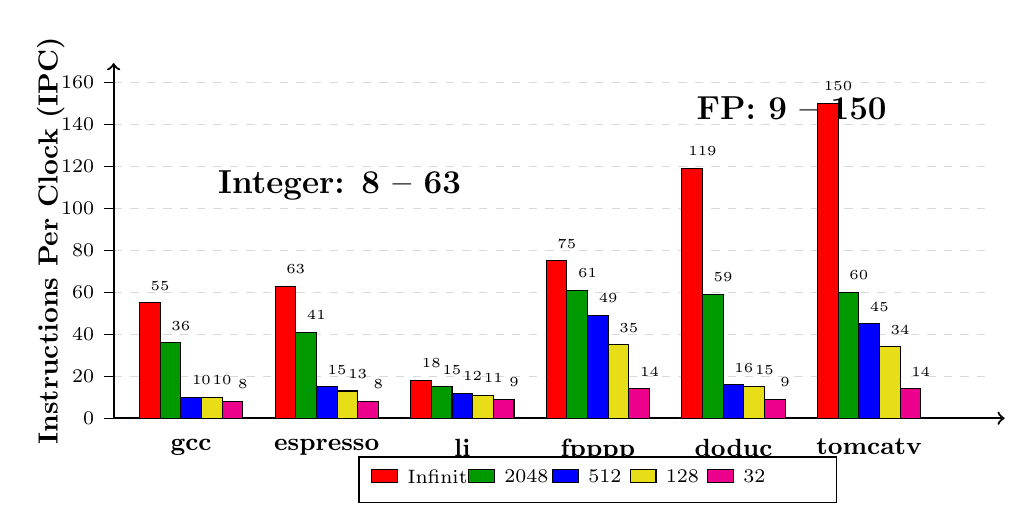
\begin{tikzpicture}[scale=0.82, font=\small]
    % Grid lines
    \draw[gray!30, dashed] (0,0) grid[ystep=0.65cm, xstep=0] (13.5, 5.2);
    
    % Axes
    \draw[->, thick] (0,0) -- (13.8, 0) node[below=14pt, midway, font=\bfseries] {Benchmarks};
    \draw[->, thick] (0,0) -- (0, 5.5) node[rotate=90, above=14pt, midway, font=\bfseries] {Instructions Per Clock (IPC)};
    
    % Y-Axis Ticks & Labels (Scale: 1 unit IPC = 0.0325 cm => 160 IPC = 5.2 cm)
    \foreach \y/\val in {0/0, 0.65/20, 1.3/40, 1.95/60, 2.6/80, 3.25/100, 3.9/120, 4.55/140, 5.2/160} {
        \draw (0, \y) -- (-0.15, \y) node[left, font=\scriptsize] {\val};
    }

    \node[font=\bfseries\large] at (3.5, 3.6) {Integer: 8 -- 63};
    \node[font=\bfseries\large] at (10.5, 4.8) {FP: 9 -- 150};

    % Bar group spacing parameters
    % Width of bar: 0.35cm. Group width: 5 * 0.35 = 1.75cm.
    
    % --- Benchmark 1: gcc --- (Inf=55, 2048=36, 512=10, 128=10, 32=8)
    \begin{scope}[shift={(0.4, 0)}]
        \draw[fill=red, draw=black] (0,0) rectangle (0.32, 1.7875) node[above=1pt, font=\tiny] {55};
        \draw[fill=green!60!black, draw=black] (0.32,0) rectangle (0.64, 1.17) node[above=1pt, font=\tiny] {36};
        \draw[fill=blue, draw=black] (0.64,0) rectangle (0.96, 0.325) node[above=1pt, font=\tiny] {10};
        \draw[fill=yellow!90!black, draw=black] (0.96,0) rectangle (1.28, 0.325) node[above=1pt, font=\tiny] {10};
        \draw[fill=magenta, draw=black] (1.28,0) rectangle (1.60, 0.26) node[above=1pt, font=\tiny] {8};
        \node[below=4pt, font=\bfseries\small] at (0.8, 0) {gcc};
    \end{scope}

    % --- Benchmark 2: espresso --- (Inf=63, 2048=41, 512=15, 128=13, 32=8)
    \begin{scope}[shift={(2.5, 0)}]
        \draw[fill=red, draw=black] (0,0) rectangle (0.32, 2.0475) node[above=1pt, font=\tiny] {63};
        \draw[fill=green!60!black, draw=black] (0.32,0) rectangle (0.64, 1.3325) node[above=1pt, font=\tiny] {41};
        \draw[fill=blue, draw=black] (0.64,0) rectangle (0.96, 0.4875) node[above=1pt, font=\tiny] {15};
        \draw[fill=yellow!90!black, draw=black] (0.96,0) rectangle (1.28, 0.4225) node[above=1pt, font=\tiny] {13};
        \draw[fill=magenta, draw=black] (1.28,0) rectangle (1.60, 0.26) node[above=1pt, font=\tiny] {8};
        \node[below=4pt, font=\bfseries\small] at (0.8, 0) {espresso};
    \end{scope}

    % --- Benchmark 3: li --- (Inf=18, 2048=15, 512=12, 128=11, 32=9)
    \begin{scope}[shift={(4.6, 0)}]
        \draw[fill=red, draw=black] (0,0) rectangle (0.32, 0.585) node[above=1pt, font=\tiny] {18};
        \draw[fill=green!60!black, draw=black] (0.32,0) rectangle (0.64, 0.4875) node[above=1pt, font=\tiny] {15};
        \draw[fill=blue, draw=black] (0.64,0) rectangle (0.96, 0.39) node[above=1pt, font=\tiny] {12};
        \draw[fill=yellow!90!black, draw=black] (0.96,0) rectangle (1.28, 0.3575) node[above=1pt, font=\tiny] {11};
        \draw[fill=magenta, draw=black] (1.28,0) rectangle (1.60, 0.2925) node[above=1pt, font=\tiny] {9};
        \node[below=4pt, font=\bfseries\small] at (0.8, 0) {li};
    \end{scope}

    % --- Benchmark 4: fpppp --- (Inf=75, 2048=61, 512=49, 128=35, 32=14)
    \begin{scope}[shift={(6.7, 0)}]
        \draw[fill=red, draw=black] (0,0) rectangle (0.32, 2.4375) node[above=1pt, font=\tiny] {75};
        \draw[fill=green!60!black, draw=black] (0.32,0) rectangle (0.64, 1.9825) node[above=1pt, font=\tiny] {61};
        \draw[fill=blue, draw=black] (0.64,0) rectangle (0.96, 1.5925) node[above=1pt, font=\tiny] {49};
        \draw[fill=yellow!90!black, draw=black] (0.96,0) rectangle (1.28, 1.1375) node[above=1pt, font=\tiny] {35};
        \draw[fill=magenta, draw=black] (1.28,0) rectangle (1.60, 0.455) node[above=1pt, font=\tiny] {14};
        \node[below=4pt, font=\bfseries\small] at (0.8, 0) {fpppp};
    \end{scope}

    % --- Benchmark 5: doduc --- (Inf=119, 2048=59, 512=16, 128=15, 32=9)
    \begin{scope}[shift={(8.8, 0)}]
        \draw[fill=red, draw=black] (0,0) rectangle (0.32, 3.8675) node[above=1pt, font=\tiny] {119};
        \draw[fill=green!60!black, draw=black] (0.32,0) rectangle (0.64, 1.9175) node[above=1pt, font=\tiny] {59};
        \draw[fill=blue, draw=black] (0.64,0) rectangle (0.96, 0.52) node[above=1pt, font=\tiny] {16};
        \draw[fill=yellow!90!black, draw=black] (0.96,0) rectangle (1.28, 0.4875) node[above=1pt, font=\tiny] {15};
        \draw[fill=magenta, draw=black] (1.28,0) rectangle (1.60, 0.2925) node[above=1pt, font=\tiny] {9};
        \node[below=4pt, font=\bfseries\small] at (0.8, 0) {doduc};
    \end{scope}

    % --- Benchmark 6: tomcatv --- (Inf=150, 2048=60, 512=45, 128=34, 32=14)
    \begin{scope}[shift={(10.9, 0)}]
        \draw[fill=red, draw=black] (0,0) rectangle (0.32, 4.875) node[above=1pt, font=\tiny] {150};
        \draw[fill=green!60!black, draw=black] (0.32,0) rectangle (0.64, 1.95) node[above=1pt, font=\tiny] {60};
        \draw[fill=blue, draw=black] (0.64,0) rectangle (0.96, 1.4625) node[above=1pt, font=\tiny] {45};
        \draw[fill=yellow!90!black, draw=black] (0.96,0) rectangle (1.28, 1.105) node[above=1pt, font=\tiny] {34};
        \draw[fill=magenta, draw=black] (1.28,0) rectangle (1.60, 0.455) node[above=1pt, font=\tiny] {14};
        \node[below=4pt, font=\bfseries\small] at (0.8, 0) {tomcatv};
    \end{scope}

    % --- Legend ---
    \begin{scope}[shift={(4.0, -1.0)}]
        \draw[fill=white, draw=black] (-0.2, -0.3) rectangle (7.2, 0.4);
        \draw[fill=red] (0,0) rectangle (0.4, 0.2);
        \node[right, font=\scriptsize] at (0.4, 0.1) {Infinite};
        
        \draw[fill=green!60!black] (1.5,0) rectangle (1.9, 0.2);
        \node[right, font=\scriptsize] at (1.9, 0.1) {2048};
        
        \draw[fill=blue] (2.8,0) rectangle (3.2, 0.2);
        \node[right, font=\scriptsize] at (3.2, 0.1) {512};
        
        \draw[fill=yellow!90!black] (4.0,0) rectangle (4.4, 0.2);
        \node[right, font=\scriptsize] at (4.4, 0.1) {128};
        
        \draw[fill=magenta] (5.2,0) rectangle (5.6, 0.2);
        \node[right, font=\scriptsize] at (5.6, 0.1) {32};
    \end{scope}

\end{tikzpicture}
\caption{Impact of Restricting Instruction Window Size on Achievable ILP.}
\label{fig:ilp_window_impact}
\end{figure}

\begin{observation}{Key Takeaways from Instruction Window Analysis}{window-impact-takeaways}
Evaluating Figure~\ref{fig:ilp_window_impact} reveals critical insights into hardware scheduling:
\begin{enumerate}
    \item \textbf{Sensitivity to Window Shrinkage:} Reducing the instruction window size from infinite down to realistic sizes (32 to 128 entries) causes a severe degradation in IPC. At a window size of 32, integer IPC falls to 8--9, while floating-point IPC drops to 9--14.
    \item \textbf{Intra-Iteration Bottlenecks:} At low window sizes, hardware cannot look far enough ahead into the instruction stream to overlap independent iterations of loops. Dependencies within single loop bodies constrain execution unless aggressive compiler optimizations (such as static loop unrolling and software pipelining) reorganize the instruction stream.
    \item \textbf{Diminishing Returns Above 2048 Entries:} Expanding the window beyond 2048 entries yields diminishing marginal returns for integer workloads, as control dependencies and address aliasing cap usable parallelism.
\end{enumerate}
\end{observation}

For subsequent experimental comparisons, standard evaluation baselines fix the instruction window size at $W = 2048$ entries and cap maximum issue capability at 64 instructions per cycle.

\section{Impact of Branch Prediction}
\label{sec:branch_impact}

In physical execution environments, branch predictors are not perfect. In our baseline setup (Instruction Window $W = 2048$, maximum issue width of 64), control dependencies severely restrict performance when branch outcomes cannot be anticipated flawlessly. To evaluate the impact of branch prediction accuracy on achievable \gls{ilp}, we compare five distinct branch prediction strategies:
\begin{enumerate}
    \item \textbf{Perfect Predictor:} Theoretical 100\% prediction accuracy (0\% misprediction rate).
    \item \textbf{Selective (Tournament) Predictor:} An 8K-entry tournament predictor that uses a selector table to dynamically choose between a 2-bit 2-level correlating predictor and a 2-bit non-correlating predictor. Across benchmarks, it achieves an average misprediction rate of approximately 3\%.
    \item \textbf{Standard 2-Bit Predictor:} A 512-entry dynamic predictor with 2-bit saturating counters.
    \item \textbf{Static (Profile-Based) Predictor:} A static predictor leveraging compiler profile data to predict the most likely branch direction.
    \item \textbf{No Predictor (None):} A conservative baseline that stalls execution at every conditional branch until the branch condition is fully resolved.
\end{enumerate}

Figure~\ref{fig:ilp_branch_impact} illustrates the achievable instructions issued per cycle under these five branch prediction schemes.

\begin{figure}[htpb]
\centering
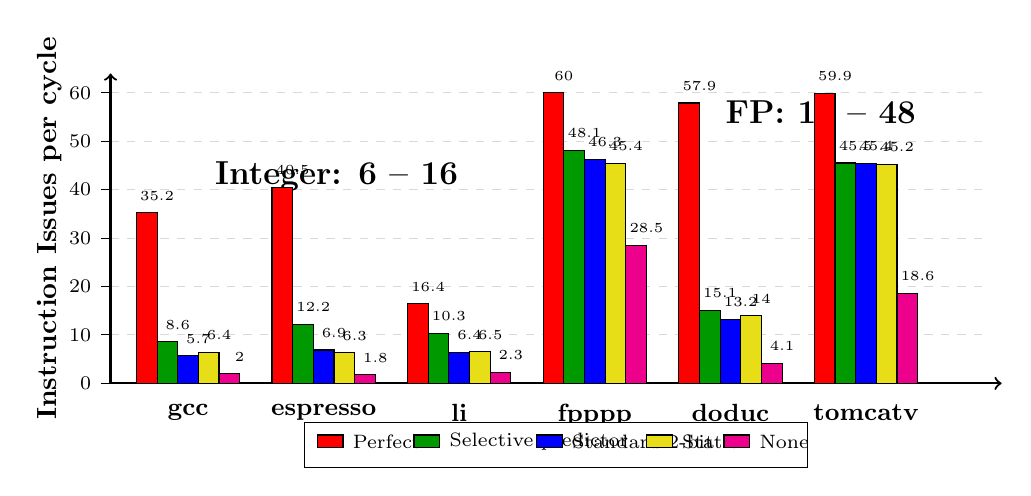
\begin{tikzpicture}[scale=0.82, font=\small]
    % Grid lines
    \draw[gray!30, dashed] (0,0) grid[ystep=0.75cm, xstep=0] (13.5, 4.5);
    
    % Axes
    \draw[->, thick] (0,0) -- (13.8, 0) node[below=14pt, midway, font=\bfseries] {Program};
    \draw[->, thick] (0,0) -- (0, 4.8) node[rotate=90, above=14pt, midway, font=\bfseries] {Instruction Issues per cycle};
    
    % Y-Axis Ticks & Labels (Scale: 1 unit IPC = 0.075 cm => 60 IPC = 4.5 cm)
    \foreach \y/\val in {0/0, 0.75/10, 1.5/20, 2.25/30, 3.0/40, 3.75/50, 4.5/60} {
        \draw (0, \y) -- (-0.15, \y) node[left, font=\scriptsize] {\val};
    }

    \node[font=\bfseries\large] at (3.5, 3.2) {Integer: 6 -- 16};
    \node[font=\bfseries\large] at (11.0, 4.2) {FP: 13 -- 48};

    % --- Benchmark 1: gcc --- (Perfect=35.2, Selective=8.6, 2-bit=5.7, Static=6.4, None=2.0)
    \begin{scope}[shift={(0.4, 0)}]
        \draw[fill=red, draw=black] (0,0) rectangle (0.32, 2.64) node[above=1pt, font=\tiny] {35.2};
        \draw[fill=green!60!black, draw=black] (0.32,0) rectangle (0.64, 0.645) node[above=1pt, font=\tiny] {8.6};
        \draw[fill=blue, draw=black] (0.64,0) rectangle (0.96, 0.4275) node[above=1pt, font=\tiny] {5.7};
        \draw[fill=yellow!90!black, draw=black] (0.96,0) rectangle (1.28, 0.48) node[above=1pt, font=\tiny] {6.4};
        \draw[fill=magenta, draw=black] (1.28,0) rectangle (1.60, 0.15) node[above=1pt, font=\tiny] {2};
        \node[below=4pt, font=\bfseries\small] at (0.8, 0) {gcc};
    \end{scope}

    % --- Benchmark 2: espresso --- (Perfect=40.5, Selective=12.2, 2-bit=6.9, Static=6.3, None=1.8)
    \begin{scope}[shift={(2.5, 0)}]
        \draw[fill=red, draw=black] (0,0) rectangle (0.32, 3.0375) node[above=1pt, font=\tiny] {40.5};
        \draw[fill=green!60!black, draw=black] (0.32,0) rectangle (0.64, 0.915) node[above=1pt, font=\tiny] {12.2};
        \draw[fill=blue, draw=black] (0.64,0) rectangle (0.96, 0.5175) node[above=1pt, font=\tiny] {6.9};
        \draw[fill=yellow!90!black, draw=black] (0.96,0) rectangle (1.28, 0.4725) node[above=1pt, font=\tiny] {6.3};
        \draw[fill=magenta, draw=black] (1.28,0) rectangle (1.60, 0.135) node[above=1pt, font=\tiny] {1.8};
        \node[below=4pt, font=\bfseries\small] at (0.8, 0) {espresso};
    \end{scope}

    % --- Benchmark 3: li --- (Perfect=16.4, Selective=10.3, 2-bit=6.4, Static=6.5, None=2.3)
    \begin{scope}[shift={(4.6, 0)}]
        \draw[fill=red, draw=black] (0,0) rectangle (0.32, 1.23) node[above=1pt, font=\tiny] {16.4};
        \draw[fill=green!60!black, draw=black] (0.32,0) rectangle (0.64, 0.7725) node[above=1pt, font=\tiny] {10.3};
        \draw[fill=blue, draw=black] (0.64,0) rectangle (0.96, 0.48) node[above=1pt, font=\tiny] {6.4};
        \draw[fill=yellow!90!black, draw=black] (0.96,0) rectangle (1.28, 0.4875) node[above=1pt, font=\tiny] {6.5};
        \draw[fill=magenta, draw=black] (1.28,0) rectangle (1.60, 0.1725) node[above=1pt, font=\tiny] {2.3};
        \node[below=4pt, font=\bfseries\small] at (0.8, 0) {li};
    \end{scope}

    % --- Benchmark 4: fpppp --- (Perfect=60.0, Selective=48.1, 2-bit=46.3, Static=45.4, None=28.5)
    \begin{scope}[shift={(6.7, 0)}]
        \draw[fill=red, draw=black] (0,0) rectangle (0.32, 4.5) node[above=1pt, font=\tiny] {60};
        \draw[fill=green!60!black, draw=black] (0.32,0) rectangle (0.64, 3.6075) node[above=1pt, font=\tiny] {48.1};
        \draw[fill=blue, draw=black] (0.64,0) rectangle (0.96, 3.4725) node[above=1pt, font=\tiny] {46.3};
        \draw[fill=yellow!90!black, draw=black] (0.96,0) rectangle (1.28, 3.405) node[above=1pt, font=\tiny] {45.4};
        \draw[fill=magenta, draw=black] (1.28,0) rectangle (1.60, 2.1375) node[above=1pt, font=\tiny] {28.5};
        \node[below=4pt, font=\bfseries\small] at (0.8, 0) {fpppp};
    \end{scope}

    % --- Benchmark 5: doduc --- (Perfect=57.9, Selective=15.1, 2-bit=13.2, Static=14.0, None=4.1)
    \begin{scope}[shift={(8.8, 0)}]
        \draw[fill=red, draw=black] (0,0) rectangle (0.32, 4.3425) node[above=1pt, font=\tiny] {57.9};
        \draw[fill=green!60!black, draw=black] (0.32,0) rectangle (0.64, 1.1325) node[above=1pt, font=\tiny] {15.1};
        \draw[fill=blue, draw=black] (0.64,0) rectangle (0.96, 0.99) node[above=1pt, font=\tiny] {13.2};
        \draw[fill=yellow!90!black, draw=black] (0.96,0) rectangle (1.28, 1.05) node[above=1pt, font=\tiny] {14};
        \draw[fill=magenta, draw=black] (1.28,0) rectangle (1.60, 0.3075) node[above=1pt, font=\tiny] {4.1};
        \node[below=4pt, font=\bfseries\small] at (0.8, 0) {doduc};
    \end{scope}

    % --- Benchmark 6: tomcatv --- (Perfect=59.9, Selective=45.5, 2-bit=45.4, Static=45.2, None=18.6)
    \begin{scope}[shift={(10.9, 0)}]
        \draw[fill=red, draw=black] (0,0) rectangle (0.32, 4.4925) node[above=1pt, font=\tiny] {59.9};
        \draw[fill=green!60!black, draw=black] (0.32,0) rectangle (0.64, 3.4125) node[above=1pt, font=\tiny] {45.5};
        \draw[fill=blue, draw=black] (0.64,0) rectangle (0.96, 3.405) node[above=1pt, font=\tiny] {45.4};
        \draw[fill=yellow!90!black, draw=black] (0.96,0) rectangle (1.28, 3.39) node[above=1pt, font=\tiny] {45.2};
        \draw[fill=magenta, draw=black] (1.28,0) rectangle (1.60, 1.395) node[above=1pt, font=\tiny] {18.6};
        \node[below=4pt, font=\bfseries\small] at (0.8, 0) {tomcatv};
    \end{scope}

    % --- Legend ---
    \begin{scope}[shift={(3.2, -1.0)}]
        \draw[fill=white, draw=black] (-0.2, -0.3) rectangle (7.6, 0.4);
        \draw[fill=red] (0,0) rectangle (0.4, 0.2);
        \node[right, font=\scriptsize] at (0.4, 0.1) {Perfect};
        
        \draw[fill=green!60!black] (1.5,0) rectangle (1.9, 0.2);
        \node[right, font=\scriptsize] at (1.9, 0.1) {Selective predictor};
        
        \draw[fill=blue] (3.4,0) rectangle (3.8, 0.2);
        \node[right, font=\scriptsize] at (3.8, 0.1) {Standard 2-bit};
        
        \draw[fill=yellow!90!black] (5.1,0) rectangle (5.5, 0.2);
        \node[right, font=\scriptsize] at (5.5, 0.1) {Static};
        
        \draw[fill=magenta] (6.3,0) rectangle (6.7, 0.2);
        \node[right, font=\scriptsize] at (6.7, 0.1) {None};
    \end{scope}

\end{tikzpicture}
\caption{Impact of Branch Prediction Schemes on Instruction Issue Rates (Window Size $W = 2048$, Max Issue = 64).}
\label{fig:ilp_branch_impact}
\end{figure}

To understand why the selective (tournament) predictor yields superior issue rates compared to standard predictors, Figure~\ref{fig:ilp_misprediction_rates} evaluates the misprediction rates across profile-based, standard 2-bit counter, and tournament prediction schemes.

\begin{figure}[htpb]
\centering
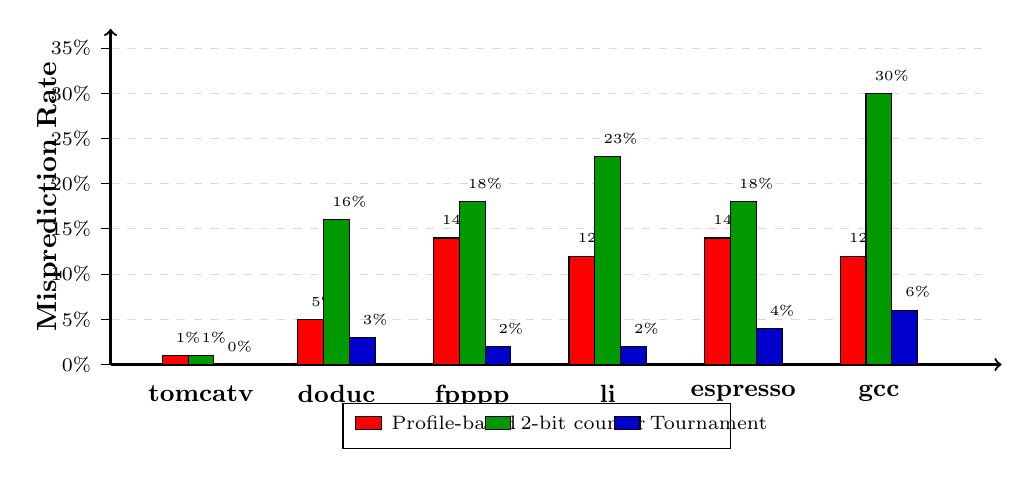
\begin{tikzpicture}[scale=0.82, font=\small]
    % Grid lines
    \draw[gray!30, dashed] (0,0) grid[ystep=0.7cm, xstep=0] (13.5, 4.9);
    
    % Axes
    \draw[->, thick] (0,0) -- (13.8, 0) node[below=14pt, midway, font=\bfseries] {Program};
    \draw[->, thick] (0,0) -- (0, 5.2) node[rotate=90, above=14pt, midway, font=\bfseries] {Misprediction Rate};
    
    % Y-Axis Ticks & Labels (Scale: 1% = 0.14 cm => 35% = 4.9 cm)
    \foreach \y/\val in {0/0\%, 0.7/5\%, 1.4/10\%, 2.1/15\%, 2.8/20\%, 3.5/25\%, 4.2/30\%, 4.9/35\%} {
        \draw (0, \y) -- (-0.15, \y) node[left, font=\scriptsize] {\val};
    }

    % Group bar width = 0.4cm. Group = 3 * 0.4 = 1.2cm.
    % --- Benchmark 1: tomcatv --- (Profile=1%, 2-bit=1%, Tournament=0%)
    \begin{scope}[shift={(0.8, 0)}]
        \draw[fill=red, draw=black] (0,0) rectangle (0.4, 0.14) node[above=1pt, font=\tiny] {1\%};
        \draw[fill=green!60!black, draw=black] (0.4,0) rectangle (0.8, 0.14) node[above=1pt, font=\tiny] {1\%};
        \draw[fill=blue!80!black, draw=black] (0.8,0) rectangle (1.2, 0.0) node[above=1pt, font=\tiny] {0\%};
        \node[below=4pt, font=\bfseries\small] at (0.6, 0) {tomcatv};
    \end{scope}

    % --- Benchmark 2: doduc --- (Profile=5%, 2-bit=16%, Tournament=3%)
    \begin{scope}[shift={(2.9, 0)}]
        \draw[fill=red, draw=black] (0,0) rectangle (0.4, 0.7) node[above=1pt, font=\tiny] {5\%};
        \draw[fill=green!60!black, draw=black] (0.4,0) rectangle (0.8, 2.24) node[above=1pt, font=\tiny] {16\%};
        \draw[fill=blue!80!black, draw=black] (0.8,0) rectangle (1.2, 0.42) node[above=1pt, font=\tiny] {3\%};
        \node[below=4pt, font=\bfseries\small] at (0.6, 0) {doduc};
    \end{scope}

    % --- Benchmark 3: fpppp --- (Profile=14%, 2-bit=18%, Tournament=2%)
    \begin{scope}[shift={(5.0, 0)}]
        \draw[fill=red, draw=black] (0,0) rectangle (0.4, 1.96) node[above=1pt, font=\tiny] {14\%};
        \draw[fill=green!60!black, draw=black] (0.4,0) rectangle (0.8, 2.52) node[above=1pt, font=\tiny] {18\%};
        \draw[fill=blue!80!black, draw=black] (0.8,0) rectangle (1.2, 0.28) node[above=1pt, font=\tiny] {2\%};
        \node[below=4pt, font=\bfseries\small] at (0.6, 0) {fpppp};
    \end{scope}

    % --- Benchmark 4: li --- (Profile=12%, 2-bit=23%, Tournament=2%)
    \begin{scope}[shift={(7.1, 0)}]
        \draw[fill=red, draw=black] (0,0) rectangle (0.4, 1.68) node[above=1pt, font=\tiny] {12\%};
        \draw[fill=green!60!black, draw=black] (0.4,0) rectangle (0.8, 3.22) node[above=1pt, font=\tiny] {23\%};
        \draw[fill=blue!80!black, draw=black] (0.8,0) rectangle (1.2, 0.28) node[above=1pt, font=\tiny] {2\%};
        \node[below=4pt, font=\bfseries\small] at (0.6, 0) {li};
    \end{scope}

    % --- Benchmark 5: espresso --- (Profile=14%, 2-bit=18%, Tournament=4%)
    \begin{scope}[shift={(9.2, 0)}]
        \draw[fill=red, draw=black] (0,0) rectangle (0.4, 1.96) node[above=1pt, font=\tiny] {14\%};
        \draw[fill=green!60!black, draw=black] (0.4,0) rectangle (0.8, 2.52) node[above=1pt, font=\tiny] {18\%};
        \draw[fill=blue!80!black, draw=black] (0.8,0) rectangle (1.2, 0.56) node[above=1pt, font=\tiny] {4\%};
        \node[below=4pt, font=\bfseries\small] at (0.6, 0) {espresso};
    \end{scope}

    % --- Benchmark 6: gcc --- (Profile=12%, 2-bit=30%, Tournament=6%)
    \begin{scope}[shift={(11.3, 0)}]
        \draw[fill=red, draw=black] (0,0) rectangle (0.4, 1.68) node[above=1pt, font=\tiny] {12\%};
        \draw[fill=green!60!black, draw=black] (0.4,0) rectangle (0.8, 4.2) node[above=1pt, font=\tiny] {30\%};
        \draw[fill=blue!80!black, draw=black] (0.8,0) rectangle (1.2, 0.84) node[above=1pt, font=\tiny] {6\%};
        \node[below=4pt, font=\bfseries\small] at (0.6, 0) {gcc};
    \end{scope}

    % --- Legend ---
    \begin{scope}[shift={(3.8, -1.0)}]
        \draw[fill=white, draw=black] (-0.2, -0.3) rectangle (5.8, 0.4);
        \draw[fill=red] (0,0) rectangle (0.4, 0.2);
        \node[right, font=\scriptsize] at (0.4, 0.1) {Profile-based};
        
        \draw[fill=green!60!black] (2.0,0) rectangle (2.4, 0.2);
        \node[right, font=\scriptsize] at (2.4, 0.1) {2-bit counter};
        
        \draw[fill=blue!80!black] (4.0,0) rectangle (4.4, 0.2);
        \node[right, font=\scriptsize] at (4.4, 0.1) {Tournament};
    \end{scope}

\end{tikzpicture}
\caption{Branch Misprediction Rates across Predictor Types.}
\label{fig:ilp_misprediction_rates}
\end{figure}

\begin{observation}{Analysis of Branch Predictor Impact}{branch-impact-analysis}
Comparing the empirical results across prediction models demonstrates:
\begin{itemize}
    \item \textbf{Dominance of Selective Prediction:} The 8K-entry selective (tournament) predictor outperforms both standard 2-bit counters and profile-based static prediction, suppressing misprediction rates to between 0\% (in numerical loops like \texttt{tomcatv}) and 6\% (in control-heavy benchmarks like \texttt{gcc}).
    \item \textbf{Performance Degradation from Branch Mispredictions:} Even a modest misprediction rate drastically reduces IPC compared to perfect prediction. In \texttt{gcc}, a 6\% misprediction rate under the selective predictor reduces performance from 35.2 IPC down to 8.6 IPC—a nearly $4\times$ throughput penalty. Similar severe drops occur in \texttt{espresso}, \texttt{doduc}, and \texttt{fpppp}.
    \item \textbf{Integer vs. Floating-Point Sensitivities:} Integer applications are constrained to 6--16 IPC under realistic branch prediction due to frequent unpredictable branches, whereas FP applications retain 13--48 IPC because loop-branch structures are highly predictable.
\end{itemize}
\end{observation}

For subsequent experimental evaluations, the baseline configuration is fixed at 256 Integer + 256 Floating-Point virtual physical registers.

\section{Impact of Memory Address Alias Analysis}
\label{sec:memory_alias_impact}

Unlike register operands whose target specifiers are known at Decode, memory dependencies are dynamic and depend on effective address calculation. To evaluate memory dependency constraints, we compare four memory alias analysis models:
\begin{enumerate}
    \item \textbf{Perfect Alias Analysis:} Ideal dynamic memory disambiguation. A memory load operation can execute speculatively ahead of any uncommitted store unless their target memory addresses actually conflict.
    \item \textbf{Global/Stack Perfect Analysis:} Perfect dynamic address disambiguation is applied to global and stack memory references. However, heap memory references are conservatively assumed to \textit{always conflict} with preceding uncommitted stores.
    \item \textbf{Inspection Analysis:} Emulates dynamic dynamic scheduling with static compiler pattern inspection. Access patterns are examined at compile time; for example, if two memory references access \texttt{20(R10)} and \texttt{100(R10)} and register \texttt{R10} is not modified between them, the compiler proves zero memory conflict. Otherwise, a conflict is assumed.
    \item \textbf{None (No Disambiguation):} All memory references are conservatively assumed to alias with every preceding uncommitted store. A load instruction must stall until all preceding store effective addresses are fully computed and resolved.
\end{enumerate}

Figure~\ref{fig:ilp_memory_alias_impact} presents the resulting IPC across integer and floating-point benchmarks under these four alias analysis models.

\begin{figure}[htpb]
\centering
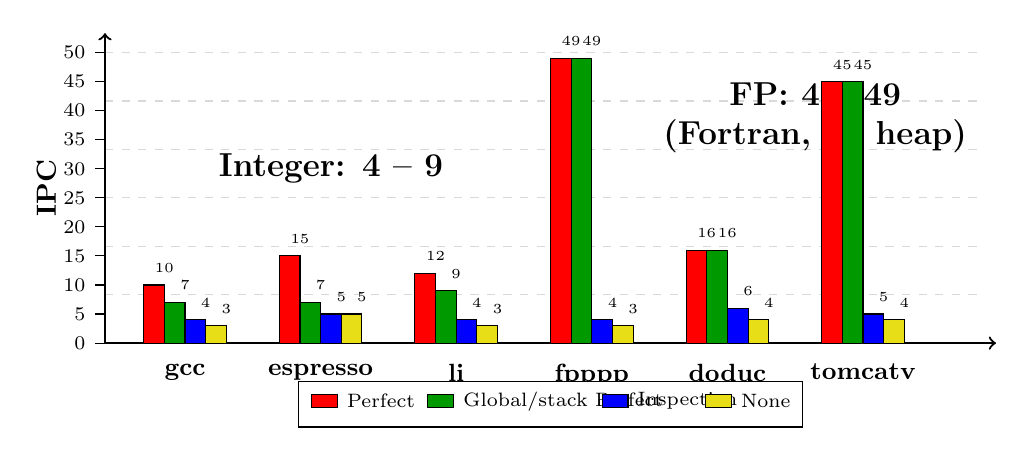
\begin{tikzpicture}[scale=0.82, font=\small]
    % Grid lines
    \draw[gray!30, dashed] (0,0) grid[ystep=0.75cm, xstep=0] (13.5, 4.5);
    
    % Axes
    \draw[->, thick] (0,0) -- (13.8, 0) node[below=14pt, midway, font=\bfseries] {Program};
    \draw[->, thick] (0,0) -- (0, 4.8) node[rotate=90, above=14pt, midway, font=\bfseries] {IPC};
    
    % Y-Axis Ticks & Labels (Scale: 1 unit IPC = 0.09 cm => 50 IPC = 4.5 cm)
    \foreach \y/\val in {0/0, 0.45/5, 0.9/10, 1.35/15, 1.8/20, 2.25/25, 2.7/30, 3.15/35, 3.6/40, 4.05/45, 4.5/50} {
        \draw (0, \y) -- (-0.15, \y) node[left, font=\scriptsize] {\val};
    }

    \node[font=\bfseries\large] at (3.5, 2.7) {Integer: 4 -- 9};
    \node[font=\bfseries\large] at (11.0, 3.5) {\begin{tabular}{c} FP: 4 -- 49 \\ (Fortran, no heap) \end{tabular}};

    % Bar group spacing parameters (4 bars per group, width=0.32cm)
    % --- Benchmark 1: gcc --- (Perfect=10, Global/Stack=7, Inspection=4, None=3)
    \begin{scope}[shift={(0.6, 0)}]
        \draw[fill=red, draw=black] (0,0) rectangle (0.32, 0.90) node[above=1pt, font=\tiny] {10};
        \draw[fill=green!60!black, draw=black] (0.32,0) rectangle (0.64, 0.63) node[above=1pt, font=\tiny] {7};
        \draw[fill=blue, draw=black] (0.64,0) rectangle (0.96, 0.36) node[above=1pt, font=\tiny] {4};
        \draw[fill=yellow!90!black, draw=black] (0.96,0) rectangle (1.28, 0.27) node[above=1pt, font=\tiny] {3};
        \node[below=4pt, font=\bfseries\small] at (0.64, 0) {gcc};
    \end{scope}

    % --- Benchmark 2: espresso --- (Perfect=15, Global/Stack=7, Inspection=5, None=5)
    \begin{scope}[shift={(2.7, 0)}]
        \draw[fill=red, draw=black] (0,0) rectangle (0.32, 1.35) node[above=1pt, font=\tiny] {15};
        \draw[fill=green!60!black, draw=black] (0.32,0) rectangle (0.64, 0.63) node[above=1pt, font=\tiny] {7};
        \draw[fill=blue, draw=black] (0.64,0) rectangle (0.96, 0.45) node[above=1pt, font=\tiny] {5};
        \draw[fill=yellow!90!black, draw=black] (0.96,0) rectangle (1.28, 0.45) node[above=1pt, font=\tiny] {5};
        \node[below=4pt, font=\bfseries\small] at (0.64, 0) {espresso};
    \end{scope}

    % --- Benchmark 3: li --- (Perfect=12, Global/Stack=9, Inspection=4, None=3)
    \begin{scope}[shift={(4.8, 0)}]
        \draw[fill=red, draw=black] (0,0) rectangle (0.32, 1.08) node[above=1pt, font=\tiny] {12};
        \draw[fill=green!60!black, draw=black] (0.32,0) rectangle (0.64, 0.81) node[above=1pt, font=\tiny] {9};
        \draw[fill=blue, draw=black] (0.64,0) rectangle (0.96, 0.36) node[above=1pt, font=\tiny] {4};
        \draw[fill=yellow!90!black, draw=black] (0.96,0) rectangle (1.28, 0.27) node[above=1pt, font=\tiny] {3};
        \node[below=4pt, font=\bfseries\small] at (0.64, 0) {li};
    \end{scope}

    % --- Benchmark 4: fpppp --- (Perfect=49, Global/Stack=49, Inspection=4, None=3)
    \begin{scope}[shift={(6.9, 0)}]
        \draw[fill=red, draw=black] (0,0) rectangle (0.32, 4.41) node[above=1pt, font=\tiny] {49};
        \draw[fill=green!60!black, draw=black] (0.32,0) rectangle (0.64, 4.41) node[above=1pt, font=\tiny] {49};
        \draw[fill=blue, draw=black] (0.64,0) rectangle (0.96, 0.36) node[above=1pt, font=\tiny] {4};
        \draw[fill=yellow!90!black, draw=black] (0.96,0) rectangle (1.28, 0.27) node[above=1pt, font=\tiny] {3};
        \node[below=4pt, font=\bfseries\small] at (0.64, 0) {fpppp};
    \end{scope}

    % --- Benchmark 5: doduc --- (Perfect=16, Global/Stack=16, Inspection=6, None=4)
    \begin{scope}[shift={(9.0, 0)}]
        \draw[fill=red, draw=black] (0,0) rectangle (0.32, 1.44) node[above=1pt, font=\tiny] {16};
        \draw[fill=green!60!black, draw=black] (0.32,0) rectangle (0.64, 1.44) node[above=1pt, font=\tiny] {16};
        \draw[fill=blue, draw=black] (0.64,0) rectangle (0.96, 0.54) node[above=1pt, font=\tiny] {6};
        \draw[fill=yellow!90!black, draw=black] (0.96,0) rectangle (1.28, 0.36) node[above=1pt, font=\tiny] {4};
        \node[below=4pt, font=\bfseries\small] at (0.64, 0) {doduc};
    \end{scope}

    % --- Benchmark 6: tomcatv --- (Perfect=45, Global/Stack=45, Inspection=5, None=4)
    \begin{scope}[shift={(11.1, 0)}]
        \draw[fill=red, draw=black] (0,0) rectangle (0.32, 4.05) node[above=1pt, font=\tiny] {45};
        \draw[fill=green!60!black, draw=black] (0.32,0) rectangle (0.64, 4.05) node[above=1pt, font=\tiny] {45};
        \draw[fill=blue, draw=black] (0.64,0) rectangle (0.96, 0.45) node[above=1pt, font=\tiny] {5};
        \draw[fill=yellow!90!black, draw=black] (0.96,0) rectangle (1.28, 0.36) node[above=1pt, font=\tiny] {4};
        \node[below=4pt, font=\bfseries\small] at (0.64, 0) {tomcatv};
    \end{scope}

    % --- Legend ---
    \begin{scope}[shift={(3.2, -1.0)}]
        \draw[fill=white, draw=black] (-0.2, -0.3) rectangle (7.6, 0.4);
        \draw[fill=red] (0,0) rectangle (0.4, 0.2);
        \node[right, font=\scriptsize] at (0.4, 0.1) {Perfect};
        
        \draw[fill=green!60!black] (1.8,0) rectangle (2.2, 0.2);
        \node[right, font=\scriptsize] at (2.2, 0.1) {Global/stack Perfect};
        
        \draw[fill=blue] (4.5,0) rectangle (4.9, 0.2);
        \node[right, font=\scriptsize] at (4.9, 0.1) {Inspection};
        
        \draw[fill=yellow!90!black] (6.1,0) rectangle (6.5, 0.2);
        \node[right, font=\scriptsize] at (6.5, 0.1) {None};
    \end{scope}

\end{tikzpicture}
\caption{Impact of Memory Address Alias Disambiguation Models on Achievable ILP.}
\label{fig:ilp_memory_alias_impact}
\end{figure}

\begin{observation}{Key Takeaways from Memory Alias Disambiguation}{memory-alias-takeaways}
Evaluating Figure~\ref{fig:ilp_memory_alias_impact} highlights distinct memory behavior across software paradigms:
\begin{itemize}
    \item \textbf{Floating-Point / Fortran Workload Characteristics:} In FORTRAN numerical floating-point benchmarks (\texttt{fpppp}, \texttt{doduc}, \texttt{tomcatv}), data is stored entirely in global static arrays or stack frames with zero dynamic heap allocation. Consequently, the Global/Stack Perfect model achieves identical performance to the Perfect alias model (49 IPC in \texttt{fpppp}, 45 IPC in \texttt{tomcatv}). However, static Inspection or None models cause performance to collapse to 3--6 IPC due to false memory dependency stalls.
    \item \textbf{Integer / C Workload Heap Reliance:} C integer programs (\texttt{gcc}, \texttt{espresso}, \texttt{li}) make extensive use of heap allocation (via \texttt{malloc}). Restricting perfect alias disambiguation to global and stack references reduces performance in \texttt{gcc} from 10 IPC down to 7 IPC, while Inspection drops performance down to 4 IPC.
\end{itemize}
\end{observation}

\section{Realistic Window Impact under Hardware Disambiguation}
\label{sec:realistic_window_impact}

Finally, we integrate all realistic hardware constraints simultaneously:
\begin{itemize}
    \item \textbf{Branch Predictor:} 8K-entry tournament (selective) branch predictor.
    \item \textbf{Register File:} 256 Integer + 256 Floating-Point physical registers.
    \item \textbf{Memory Disambiguation:} Dynamic hardware memory address alias disambiguation.
\end{itemize}

Under these cumulative constraints, we vary the Instruction Window Size across eight configurations: Infinite, 256, 128, 64, 32, 16, 8, and 4 instructions. Figure~\ref{fig:ilp_realistic_window_impact} summarizes the achievable IPC.

\begin{figure}[htpb]
\centering
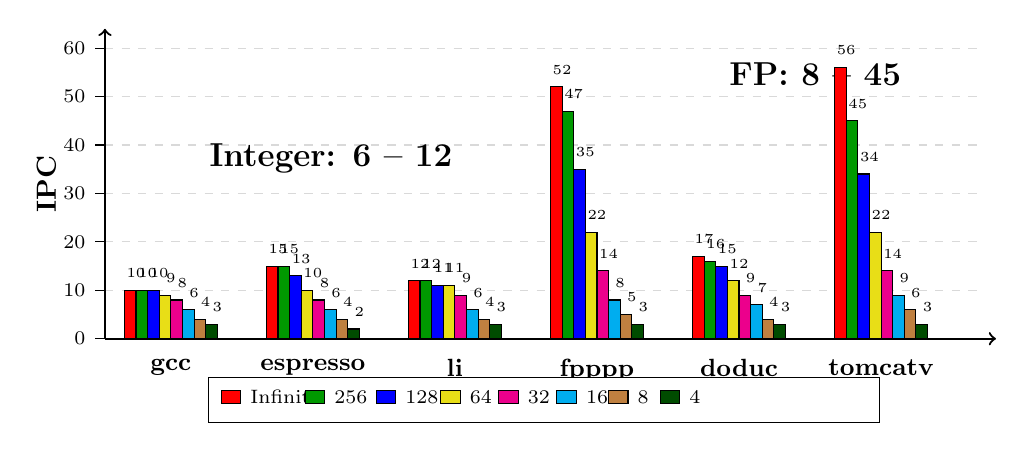
\begin{tikzpicture}[scale=0.82, font=\small]
    % Grid lines
    \draw[gray!30, dashed] (0,0) grid[ystep=0.75cm, xstep=0] (13.5, 4.5);
    
    % Axes
    \draw[->, thick] (0,0) -- (13.8, 0) node[below=14pt, midway, font=\bfseries] {Program};
    \draw[->, thick] (0,0) -- (0, 4.8) node[rotate=90, above=14pt, midway, font=\bfseries] {IPC};
    
    % Y-Axis Ticks & Labels (Scale: 1 unit IPC = 0.075 cm => 60 IPC = 4.5 cm)
    \foreach \y/\val in {0/0, 0.75/10, 1.5/20, 2.25/30, 3.0/40, 3.75/50, 4.5/60} {
        \draw (0, \y) -- (-0.15, \y) node[left, font=\scriptsize] {\val};
    }

    \node[font=\bfseries\large] at (3.5, 2.8) {Integer: 6 -- 12};
    \node[font=\bfseries\large] at (11.0, 4.1) {FP: 8 -- 45};

    % Bar group spacing parameters (8 bars per group, width=0.18cm)
    % --- Benchmark 1: gcc --- (Inf=10, 256=10, 128=10, 64=9, 32=8, 16=6, 8=4, 4=3)
    \begin{scope}[shift={(0.3, 0)}]
        \draw[fill=red, draw=black] (0,0) rectangle (0.18, 0.75) node[above=1pt, font=\tiny] {10};
        \draw[fill=green!60!black, draw=black] (0.18,0) rectangle (0.36, 0.75) node[above=1pt, font=\tiny] {10};
        \draw[fill=blue, draw=black] (0.36,0) rectangle (0.54, 0.75) node[above=1pt, font=\tiny] {10};
        \draw[fill=yellow!90!black, draw=black] (0.54,0) rectangle (0.72, 0.675) node[above=1pt, font=\tiny] {9};
        \draw[fill=magenta, draw=black] (0.72,0) rectangle (0.90, 0.60) node[above=1pt, font=\tiny] {8};
        \draw[fill=cyan, draw=black] (0.90,0) rectangle (1.08, 0.45) node[above=1pt, font=\tiny] {6};
        \draw[fill=brown, draw=black] (1.08,0) rectangle (1.26, 0.30) node[above=1pt, font=\tiny] {4};
        \draw[fill=green!30!black, draw=black] (1.26,0) rectangle (1.44, 0.225) node[above=1pt, font=\tiny] {3};
        \node[below=4pt, font=\bfseries\small] at (0.72, 0) {gcc};
    \end{scope}

    % --- Benchmark 2: espresso --- (Inf=15, 256=15, 128=13, 64=10, 32=8, 16=6, 8=4, 4=2)
    \begin{scope}[shift={(2.5, 0)}]
        \draw[fill=red, draw=black] (0,0) rectangle (0.18, 1.125) node[above=1pt, font=\tiny] {15};
        \draw[fill=green!60!black, draw=black] (0.18,0) rectangle (0.36, 1.125) node[above=1pt, font=\tiny] {15};
        \draw[fill=blue, draw=black] (0.36,0) rectangle (0.54, 0.975) node[above=1pt, font=\tiny] {13};
        \draw[fill=yellow!90!black, draw=black] (0.54,0) rectangle (0.72, 0.75) node[above=1pt, font=\tiny] {10};
        \draw[fill=magenta, draw=black] (0.72,0) rectangle (0.90, 0.60) node[above=1pt, font=\tiny] {8};
        \draw[fill=cyan, draw=black] (0.90,0) rectangle (1.08, 0.45) node[above=1pt, font=\tiny] {6};
        \draw[fill=brown, draw=black] (1.08,0) rectangle (1.26, 0.30) node[above=1pt, font=\tiny] {4};
        \draw[fill=green!30!black, draw=black] (1.26,0) rectangle (1.44, 0.15) node[above=1pt, font=\tiny] {2};
        \node[below=4pt, font=\bfseries\small] at (0.72, 0) {espresso};
    \end{scope}

    % --- Benchmark 3: li --- (Inf=12, 256=12, 128=11, 64=11, 32=9, 16=6, 8=4, 4=3)
    \begin{scope}[shift={(4.7, 0)}]
        \draw[fill=red, draw=black] (0,0) rectangle (0.18, 0.90) node[above=1pt, font=\tiny] {12};
        \draw[fill=green!60!black, draw=black] (0.18,0) rectangle (0.36, 0.90) node[above=1pt, font=\tiny] {12};
        \draw[fill=blue, draw=black] (0.36,0) rectangle (0.54, 0.825) node[above=1pt, font=\tiny] {11};
        \draw[fill=yellow!90!black, draw=black] (0.54,0) rectangle (0.72, 0.825) node[above=1pt, font=\tiny] {11};
        \draw[fill=magenta, draw=black] (0.72,0) rectangle (0.90, 0.675) node[above=1pt, font=\tiny] {9};
        \draw[fill=cyan, draw=black] (0.90,0) rectangle (1.08, 0.45) node[above=1pt, font=\tiny] {6};
        \draw[fill=brown, draw=black] (1.08,0) rectangle (1.26, 0.30) node[above=1pt, font=\tiny] {4};
        \draw[fill=green!30!black, draw=black] (1.26,0) rectangle (1.44, 0.225) node[above=1pt, font=\tiny] {3};
        \node[below=4pt, font=\bfseries\small] at (0.72, 0) {li};
    \end{scope}

    % --- Benchmark 4: fpppp --- (Inf=52, 256=47, 128=35, 64=22, 32=14, 16=8, 8=5, 4=3)
    \begin{scope}[shift={(6.9, 0)}]
        \draw[fill=red, draw=black] (0,0) rectangle (0.18, 3.90) node[above=1pt, font=\tiny] {52};
        \draw[fill=green!60!black, draw=black] (0.18,0) rectangle (0.36, 3.525) node[above=1pt, font=\tiny] {47};
        \draw[fill=blue, draw=black] (0.36,0) rectangle (0.54, 2.625) node[above=1pt, font=\tiny] {35};
        \draw[fill=yellow!90!black, draw=black] (0.54,0) rectangle (0.72, 1.65) node[above=1pt, font=\tiny] {22};
        \draw[fill=magenta, draw=black] (0.72,0) rectangle (0.90, 1.05) node[above=1pt, font=\tiny] {14};
        \draw[fill=cyan, draw=black] (0.90,0) rectangle (1.08, 0.60) node[above=1pt, font=\tiny] {8};
        \draw[fill=brown, draw=black] (1.08,0) rectangle (1.26, 0.375) node[above=1pt, font=\tiny] {5};
        \draw[fill=green!30!black, draw=black] (1.26,0) rectangle (1.44, 0.225) node[above=1pt, font=\tiny] {3};
        \node[below=4pt, font=\bfseries\small] at (0.72, 0) {fpppp};
    \end{scope}

    % --- Benchmark 5: doduc --- (Inf=17, 256=16, 128=15, 64=12, 32=9, 16=7, 8=4, 4=3)
    \begin{scope}[shift={(9.1, 0)}]
        \draw[fill=red, draw=black] (0,0) rectangle (0.18, 1.275) node[above=1pt, font=\tiny] {17};
        \draw[fill=green!60!black, draw=black] (0.18,0) rectangle (0.36, 1.20) node[above=1pt, font=\tiny] {16};
        \draw[fill=blue, draw=black] (0.36,0) rectangle (0.54, 1.125) node[above=1pt, font=\tiny] {15};
        \draw[fill=yellow!90!black, draw=black] (0.54,0) rectangle (0.72, 0.90) node[above=1pt, font=\tiny] {12};
        \draw[fill=magenta, draw=black] (0.72,0) rectangle (0.90, 0.675) node[above=1pt, font=\tiny] {9};
        \draw[fill=cyan, draw=black] (0.90,0) rectangle (1.08, 0.525) node[above=1pt, font=\tiny] {7};
        \draw[fill=brown, draw=black] (1.08,0) rectangle (1.26, 0.30) node[above=1pt, font=\tiny] {4};
        \draw[fill=green!30!black, draw=black] (1.26,0) rectangle (1.44, 0.225) node[above=1pt, font=\tiny] {3};
        \node[below=4pt, font=\bfseries\small] at (0.72, 0) {doduc};
    \end{scope}

    % --- Benchmark 6: tomcatv --- (Inf=56, 256=45, 128=34, 64=22, 32=14, 16=9, 8=6, 4=3)
    \begin{scope}[shift={(11.3, 0)}]
        \draw[fill=red, draw=black] (0,0) rectangle (0.18, 4.20) node[above=1pt, font=\tiny] {56};
        \draw[fill=green!60!black, draw=black] (0.18,0) rectangle (0.36, 3.375) node[above=1pt, font=\tiny] {45};
        \draw[fill=blue, draw=black] (0.36,0) rectangle (0.54, 2.55) node[above=1pt, font=\tiny] {34};
        \draw[fill=yellow!90!black, draw=black] (0.54,0) rectangle (0.72, 1.65) node[above=1pt, font=\tiny] {22};
        \draw[fill=magenta, draw=black] (0.72,0) rectangle (0.90, 1.05) node[above=1pt, font=\tiny] {14};
        \draw[fill=cyan, draw=black] (0.90,0) rectangle (1.08, 0.675) node[above=1pt, font=\tiny] {9};
        \draw[fill=brown, draw=black] (1.08,0) rectangle (1.26, 0.45) node[above=1pt, font=\tiny] {6};
        \draw[fill=green!30!black, draw=black] (1.26,0) rectangle (1.44, 0.225) node[above=1pt, font=\tiny] {3};
        \node[below=4pt, font=\bfseries\small] at (0.72, 0) {tomcatv};
    \end{scope}

    % --- Legend ---
    \begin{scope}[shift={(1.8, -1.0)}]
        \draw[fill=white, draw=black] (-0.2, -0.3) rectangle (10.2, 0.4);
        \draw[fill=red] (0,0) rectangle (0.3, 0.2);
        \node[right, font=\scriptsize] at (0.3, 0.1) {Infinite};
        
        \draw[fill=green!60!black] (1.3,0) rectangle (1.6, 0.2);
        \node[right, font=\scriptsize] at (1.6, 0.1) {256};
        
        \draw[fill=blue] (2.4,0) rectangle (2.7, 0.2);
        \node[right, font=\scriptsize] at (2.7, 0.1) {128};
        
        \draw[fill=yellow!90!black] (3.4,0) rectangle (3.7, 0.2);
        \node[right, font=\scriptsize] at (3.7, 0.1) {64};
        
        \draw[fill=magenta] (4.3,0) rectangle (4.6, 0.2);
        \node[right, font=\scriptsize] at (4.6, 0.1) {32};

        \draw[fill=cyan] (5.2,0) rectangle (5.5, 0.2);
        \node[right, font=\scriptsize] at (5.5, 0.1) {16};

        \draw[fill=brown] (6.0,0) rectangle (6.3, 0.2);
        \node[right, font=\scriptsize] at (6.3, 0.1) {8};

        \draw[fill=green!30!black] (6.8,0) rectangle (7.1, 0.2);
        \node[right, font=\scriptsize] at (7.1, 0.1) {4};
    \end{scope}

\end{tikzpicture}
\caption{Realistic Window Size Impact under Combined Hardware Constraints (8K Tournament Branch Predictor, 256 Registers, Hardware Alias Disambiguation).}
\label{fig:ilp_realistic_window_impact}
\end{figure}

\begin{observation}{Curved Drop Off in Realistic Parallelism}{realistic-window-takeaways}
As shown in Figure~\ref{fig:ilp_realistic_window_impact}, introducing realistic branch prediction, register renaming, and memory disambiguation creates a characteristic "curved" degradation profile:
\begin{itemize}
    \item \textbf{Integer Benchmark Saturation (6 -- 12 IPC):} Integer applications (\texttt{gcc}, \texttt{espresso}, \texttt{li}) saturate early. Performance drops slightly from Infinite down to 256 entries, remains relatively stable between 256 and 128 entries (10--12 IPC), and drops steeply once the window shrinks below 64 entries.
    \item \textbf{Floating-Point Sensitivity (8 -- 45 IPC):} Floating-point workloads exhibit sharp performance drops at every window size boundary (e.g., \texttt{tomcatv} drops from 56 IPC down to 45 IPC at 256 entries, 34 IPC at 128 entries, and 22 IPC at 64 entries).
\end{itemize}
\end{observation}

\section{Summary and Practical Bounds on Achievable ILP}
\label{sec:summary_ilp_bounds}

Understanding the limits of Instruction-Level Parallelism provides crucial design guidelines for microarchitects and compiler authors:

\begin{concept}{Practical Architectural Limitations}{practical-ilp-limits}
\begin{enumerate}
    \item \textbf{Optimistic Assumptions vs. Physical Realities:}
    \begin{itemize}
        \item Ideal studies assume unrestricted multi-issue execution across all instructions. However, if a window contains a cluster composed entirely of memory references, structural pipeline hazards and cache port contention serialize execution.
        \item Non-ideal caches introduce multi-cycle hit/miss penalties, while complex functional units (such as floating-point dividers or vector pipelines) exhibit multi-cycle non-unit execution latencies.
    \end{itemize}
    \item \textbf{Window Size Impact on Integer Programs:}
    \begin{itemize}
        \item Instruction window size has a significantly smaller relative impact on integer programs than on numerical floating-point code. Branch misprediction penalties, pointer chasing, and limited baseline instruction-level parallelism cap integer throughput well before window capacity becomes the primary bottleneck.
    \end{itemize}
    \item \textbf{Evolution of Processing Paradigms:}
    \begin{itemize}
        \item Over recent decades, industry focus shifted heavily toward integer and irregular data structures.
        \item Rather than pushing for unfeasible single-thread ILP bounds via ultra-wide dynamic instruction windows, modern high-performance microarchitectures embrace domain-specific hardware, wide \glsfmtshort{simd} vector extensions, and data-parallel accelerator architectures (GPUs/TPUs) to drive machine learning and high-throughput computing performance curves.
    \end{itemize}
\end{enumerate}
\end{concept}